%!TEX root = ../main.tex

\chapter{System Arkitektur}

\RevisionsTabel{System Arkitektur}{
Alle	& 1.0	& 17-03-2015  \\
		& 	 	&   \\
		& 		&   \\
		& 	 	&   \\
}

Dette afsnit beskriver systemarkitekturen for systemet \gls{AVS}, som er specificeret i kravspecifikation. Her anvendes SysML til beskrivelse af struktur og interaktion imellem komponenterne. Fastlæggelse af grænseflader mellem systemets komponenter og beskrivelse af disse.

\begin{figure}[H]
    \centering
    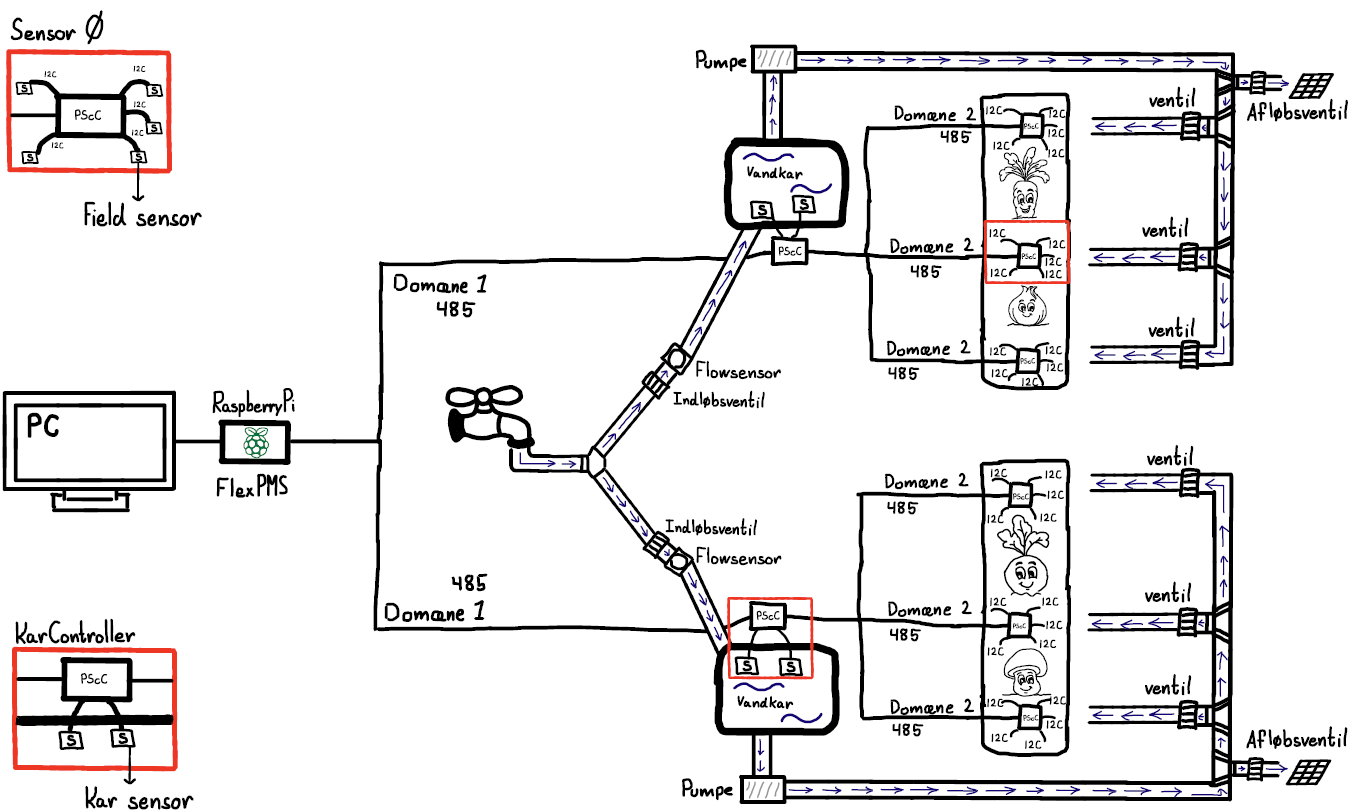
\includegraphics[width=\textwidth]{SystemArkitektur/AVS}
    \caption{Grafisk systembeskrivelse}
    \label{fig:graf_sys}
\end{figure}
Figur \ref{fig:graf_sys}, er en grafisk systembeskrivelse af det overordnede system som har indholder følgende:
\begin{itemize}
\item De blå pile illustrer vandvejen gennem vandslanger i forhold til kar, ventiler og pumpen. 
\item Ud fra var vandkaret sider en PSoC, som er forbundet til sensorerne på karet og de PSoC's der ligger i gromediet/plantekasserne.
\item I plantekasserne ligger der nogle PSoC's som bliver kaldt for \glslink{sensoroe}{Sensor Øer}, disse er forbundet til nogle sensorer der tager nogle forskellige målinger. 
\end{itemize}
\section{System diagrammer}
\fxnote{Der skal laves software diagrammer til system arkitektur - applikationsmodel sekvens diagrammer state machines osv. }

%!TEX root = ../../main.tex

\subsection{System Domænemodel}

\begin{figure}[H]
	\centering
	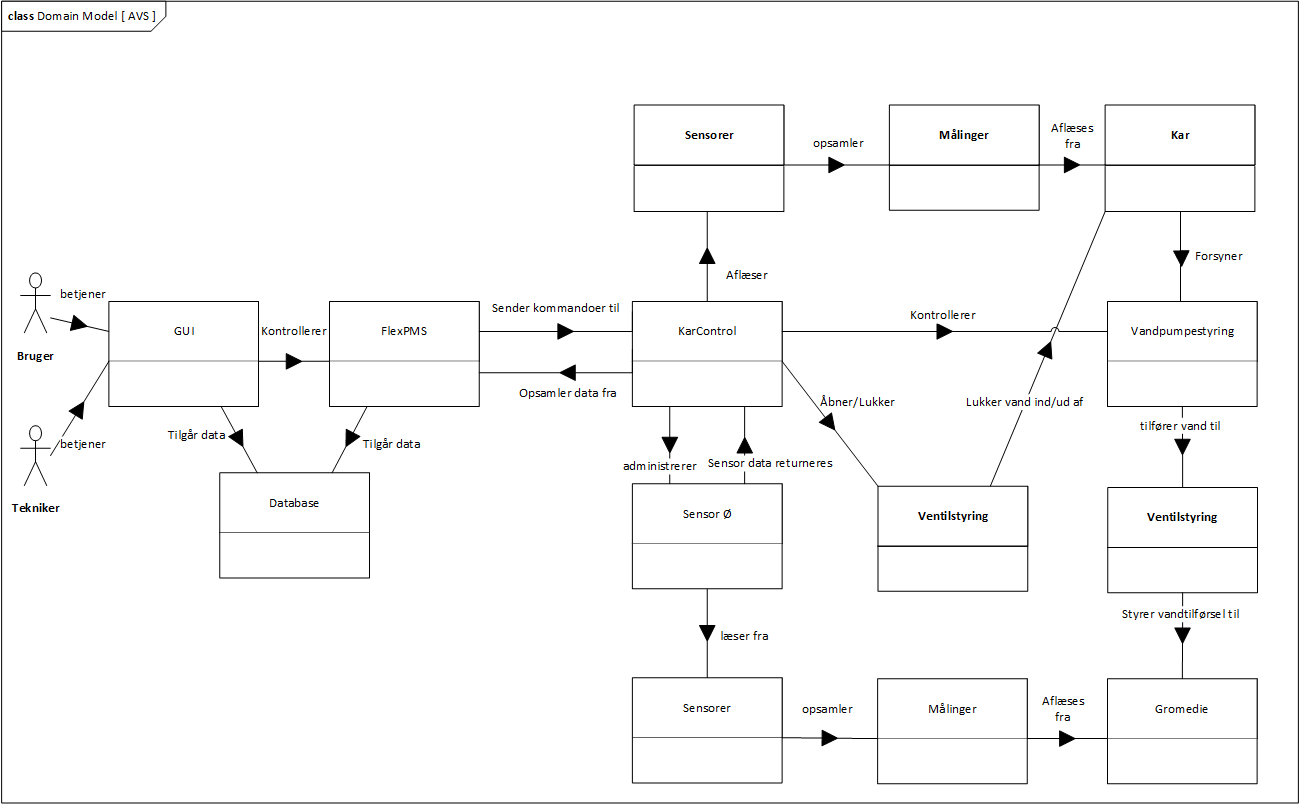
\includegraphics[width=0.82\textwidth]{Systemarkitektur/System/AVS_domain_model.png}
	\label{fig:System BDD}
	\caption{Domain model af AVS}
\end{figure}



\subsection{System BDD}

\begin{figure}[H]
	\centering
	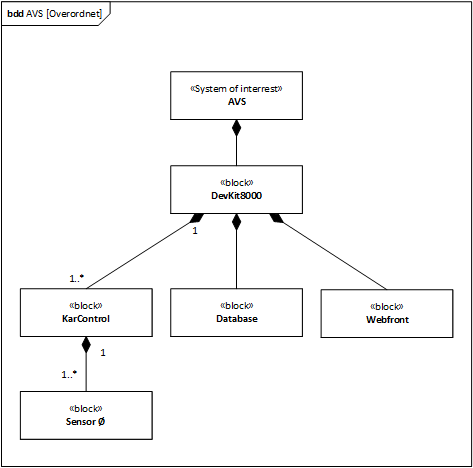
\includegraphics[width=0.82\textwidth]{Systemarkitektur/System/AVS_SystemdiagramBDD.png}
	\label{fig:System BDD}
	\caption{Block Definition Diagram af AVS}
\end{figure}



\subsection{Allokeringsdiagram}

\begin{figure}[H]
	\centering
	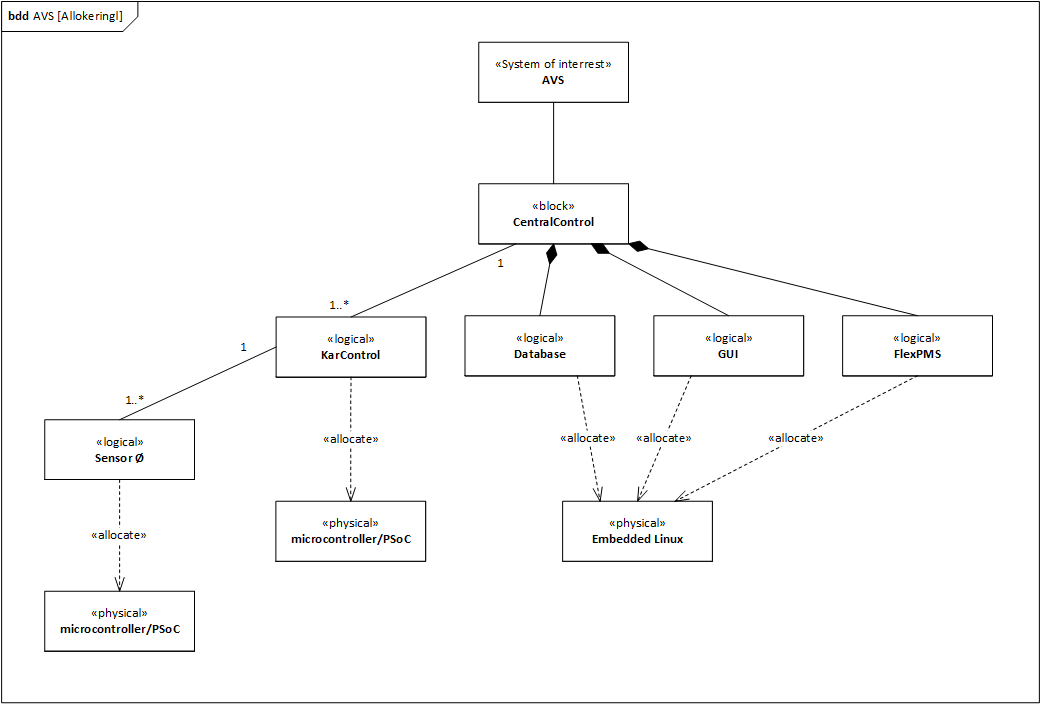
\includegraphics[width=0.82\textwidth]{Systemarkitektur/System/AVS_Allokeringsdiagram.png}
	\label{fig:System BDD}
	\caption{Allokeringsdiagram af AVS}
\end{figure}









\newpage
\section{CentralControl diagrammer}
\subsection{CentralControl IBD}
\systemIBD{0.82}{CentralControl}{CentralControl}

\subsection{Signal beskrivelser}
\systemSignaler{CentralControl} {
KarBus				& RS485 bus til kommunikation mellem enheder &	 	& Differentielt bussystem  \\
Data485				& RS485 bus til kommunikation mellem enheder &	 	& internt signal   \\
Data232				& RS485 konverteret til UART 232			 &	 	& Signal efter konvertering  \\
PMSConn				& Database forbindelse						 &		& Til at skrive log \\
GUIConn				& Database forbindelse						 &		& Til at hente og skrive indstillinger samt log \\
ControlConn			& Socket forbindelse fra GUI til FlexPMS	 &		& Til at sende kommandoer fra GUI til FlexPMS \\
html				& Http protokol								 &		& Fobindelse til brugerens browser \\
}

\newpage
\section{KarControl diagrammer}
%!TEX root = ../../main.tex

\subsection{KarControl BDD}
\systemBDD{0.82}{KarControl}

\subsubsection{KarGruppe}
KarGruppe er den overordnede betegnelse for et vandkar med tilførende pH-værdi og gødningskoncentration. KarGruppen består af diverse sensorer og aktuatorer, og styrer et vilkårligt antal Sensor Ø’er. KarGruppen er styret af en controller, KarControl.

\subsubsection{Indløbsventil}
Indløbsventilen åbner og lukker for vandtilføjelsen til karret. Den bruges i forbindelse med, at der skal fyldes vand på karret. Det antages, at indløbsventilen er tilsluttet en vandforsyning, som altid er åben.

\subsubsection{Afløbsventil}
Afløbsventilen åbner og lukker for, at vand kan løbe ud af karret. Den bruges i forbindelse med, at karret skal tømmes.

\subsubsection{pH-Sensor}
pH-sensoren målet pH-værdien af gødningsblandingen i karret.

\subsubsection{Vandpumpe}
Vandpumpen pumper vand fra karret ud til Sensor Ø’erne.

\subsubsection{Flowmåler}
Flowmåleren måler mængden af vand, som tilføres karret gennem Indløbsventilen.

\subsubsection{PSU}
PSU (Power Supply Unit) forsyner de andre blokke med 12V og 5V.

\subsection{KarControl IBD}
\systemIBD{0.82}{KarControl}{KarControl}

\subsubsection{RSIn}
RSConverter konverterer mellem RS485 og UART 232 når der skal kommunikeres med CentralControl.

\subsubsection{RSOut}
RSConverter konverterer mellem RS485 og UART 232 når der skal kommunikeres med Sensor Ø'er.

\subsection{KarControlForsyning IBD}
Der er lavet et separat forsynings IBD som viser forbindelserne fra blokken PSU til resten af blokkene og omverdenen.
\begin{figure}[H]
	\centering
	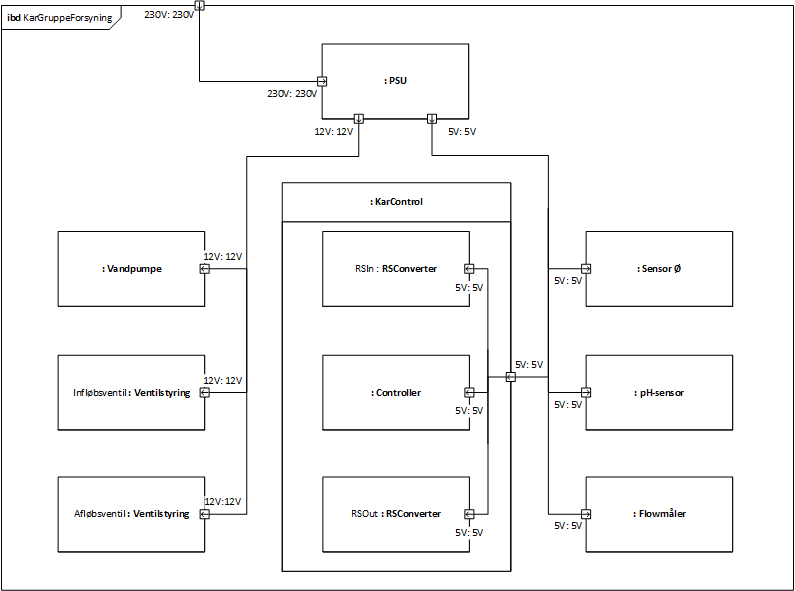
\includegraphics[scale=0.7]{Systemarkitektur/KarControl/KarControlForsyning_IBD.png}
	\label{fig:KarControlForsyning}
	\caption{IBD over forsyningsforbindelser til KarControl}
\end{figure}

%\subsection{KarControl Allokeringsdiagram}
%\systemAllokeringsDiagram{0.82}{KarControl}{KarControl}

\subsection{Signalbeskrivelser KarControl}
\systemSignaler{KarControl} {
KarBus				& RS485 bus til kommunikation mellem enheder &	 	& Differentielt bussystem  \\
OeBus				& RS485 bus til kommunikation mellem enheder &	 	& Differentielt bussystem  \\
Data485				& RS485 bus til kommunikation mellem enheder &	 	& internt signal   \\
Data232				& RS485 konverteret til logisk niveau		 &	 	& Signal efter konvertering  \\
EnableIndløb		& Signal til at lukke vand ind i kar		 & 0-5V	& Signal til at styre magnetventil   \\
EnableAfløb			& Signal til at lukke vand ud af kar		 & 0-5V	& Signal til at styre magnetventil	\\
EnableVandpumpe		& Signal til styring af vandpumpe			   	     & 0-5V & PWM styret signal	\\
Puls				& Takttæller af flow				   	 	 & 0-5V & 	\\
pH					& Analog signal fra pH måler			 	 & fra -420 til 420 mV  & Analogt signal	\\
Indløb				& vandstyring i kar							 &    	& Til at lukke vand ind i kar	\\
Afløb				& vandstyring i kar	 						 &   	& Til at lukke vand ud af kar	\\
Dossering			& vandstyring til planter					 &      & Til at dosere vand til planterne	\\
230V				& El-nettet som forsyner PSU				 & 230V	& \\
12V					& Forsyning til pumper og ventiler			 & 12V	& \\
5V					& Forsyning til systemets logiske kredsløb	 & 5V	& \\
}

\newpage
\section{Sensor Ø diagrammer}
%!TEX root = ../../main.tex

\subsection{Sensor Ø BDD}
\systemBDD[Sensor_oe]{0.82}{Sensor Ø}

\subsubsection*{Sensor Ø Control}
Sensor Ø Control tager imod kommandoer fra KarControl, som instruerer omkring åbning og lukning af Doseringsventil. KarControl anmoder også om, at Sensor Ø Control skal sende måledata fra sensors, som er tilkoblet Sensor Ø’en.

\subsubsection{Doseringsventil}
Doseringsventilen åbner og lukker for vandtilførslen til planterne i området omkring Sensor Ø’en, som Doseringsventilen er tilkoblet. Når KarControl tænder for Vandpumpen kan de enkelte Sensor Ø’ers Doseringsventiler være åbne eller lukkede alt efter, om planterne omkring Sensor Ø’en har brug for vand.

\subsubsection{Fieldsensor}
Fieldsensor er en generalisering af alle slags sensorer, som kan tilsluttes Sensor Ø’en. Vilkårligt mange sensorer kan tilkobles en bus, og kommunikere med Sensor Ø Control gennem en standardiseret protokol. Sensor kan kun aflevere målinger når de bliver bedt om at levere dem.

\subsection{Sensor Ø IBD}
\systemIBD{0.82}{Sensor_oe}{Sensor Ø}

%\subsection{Sensor Ø Allokeringsdiagram}
%\systemAllokeringsDiagram{0.82}{Sensor_oe}{Sensor Ø}

\subsection{Signal beskrivelser}
\systemSignaler[SensorOe]{Sensor Ø}{
oeData				& Buskommunikation efter konvertering fra 485 &	 	& UART kommunikation fra 485 bussen  \\
oeBus				& RS485 bus til kommunikation mellem enheder  &	 	& Differentielt bussystem  \\
sensorData			& Signal på I2C bus							  &	 	& Kan være flere forskellige signaler alt efter sensor type   \\
ventilCtrl			& Signal til styring af doserings ventil	  &	0-5V& Bruges til at styre mængden af vand til planterne \\
vand				& Dette er flow'et af vand 					  &		& \\
}

\newpage
\section{Fieldsensor diagrammer}
%!TEX root = ../../main.tex

\subsection{Fieldsensor BDD}
Dette er vores modelLibrary af de sensorer der matcher Fieldsensor specifikationerne

\systemBDD{0.7}{Fieldsensor}

\subsection{Signalbeskrivelser Fieldsenser}
\systemSignaler{Fieldsensor}{
sensorData				&  I2C kommunikation			& Logisk: 0-5V 	&  Kommunikation fra sensorer til Fieldsensor\\
}

\newpage
\section{Jordfugt sensor diagrammer}
%!TEX root = ../../main.tex

Jordfugt sensoren måler en strøm igennem jorden. Denne strøm vil variere med hensyn til fugtigheden som derfor vil resultere i en spændingsændring på indgangen af analog til digital konverteren. Denne spænding bruges til at udregne fugtigheden i procent

\subsection{Jordfugt sensor BDD}
\systemBDD[Sensor_Jordfugt]{0.83}{Jordfugt sensor}

\subsection{Jordfugt sensor IBD}
\systemIBD{0.83}{Sensor_Jordfugt}{Jordfugt sensor}

\subsection{Signalbeskrivelser Jordfugtighedssensor}
\systemSignaler{Jordfugt sensor}{
Målespænding		& Spændingsforskel 				& 	 				& Differential spænding skab af fugtighed i jorden  	 \\
DataADC				& ADC-konverteret målespænding 	& Logisk: 0-5V	 	& Digitalt konverteret målesignal   					 \\
DataI2C				& I2C kommunikation 			& Logisk: 0-5V	 	& Kommunikation fra Jordfugtighedsmåler til Fieldsensor  \\
}

\newpage
\section{pH-sensor diagrammer}
%!TEX root = ../../main.tex

Til pH måling har vi bygget vores egen sensor ved hjælp af en pH-probe.

\subsection{pH-sensor BDD}

I forhold til signaler er proben ret nem at have med at gøre da den selv producere en spænding i forhold til den væske der måles på pH værdi.

\begin{figure}[H]
	\centering
	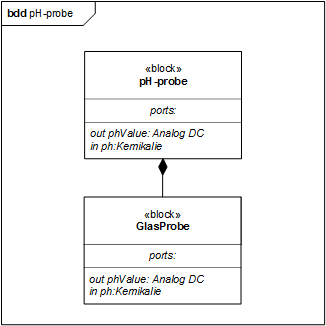
\includegraphics[width=0.7\textwidth]{Systemarkitektur/Sensor_pH/pH_Probe_BDD.png}
	\label{fig:pH-sensor BDD}
	\caption{Block Definition Diagram af pH-sensor}
\end{figure}



\subsection{pH-sensor IBD}

Igen ses simpliciteten da pH proben bare interagere med kemikalium og herefter producere en spænding.

\begin{figure}[H]
	\centering
	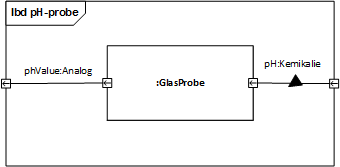
\includegraphics[width=0.7\textwidth]{Systemarkitektur/Sensor_pH/pH_Probe_IBD.png}
	\label{fig:pH-sensor IBD}
	\caption{Internal Block Diagram af pH-sensor}
\end{figure}




\newpage
\section{Ventilstyring diagrammer}
%!TEX root = ../../main.tex

Da vi bruger ventiler flere steder i systemet er dette en general beskrivelse af dem.

\subsection{Ventilstyring BDD}

Her under ses et diagram over den generalle opbygning af ventil styringen denne gør sig gældende for alle ventilerne i systemet

\systemBDD{0.5}{Ventilstyring}{Ventilstyring}

Her ses så de interne forbindelser i Ventilstyringen 

\subsection{Ventilstyring IBD}

Her ses så de interne forbindelser i Ventilstyringen 

\systemIBD{0.5}{Ventilstyring}{Ventilstyring}



\newpage
\section{Vandpumpestyring diagrammer}
%!TEX root = ../../main.tex

Vi bruger en vandpumpe på alle vores kar.

\subsection{Vandpumpestyring BDD}
Her under ses et diagram over den generalle opbygning af vandpumpe styringen denne gør sig gældende for alle vandpumper i systemet

\systemBDD{0.5}{Vandpumpestyring}

\subsection{Vandpumpestyring IBD}
Her ses så de interne forbindelser i Vandpumpestyringen 

\systemIBD{0.5}{Vandpumpestyring}{Vandpumpestyring}

\subsection{Signal beskrivelser}
\systemSignaler{Vandpumpestyring}{
cV				& Pwm signal til Mosfet kredsløbet 			&	0-5V 		&  Bestemmer om Vandpumpen roterer \\
vand			& Vand der flyder gennem Vandpumpen			& 0 - 17l/min	& Bestemmer mængden af vand til dosering	\\
}

\newpage
\section{Teknologiundersøgelser}
%!TEX root = ../../main.tex
%!TEX root = ../../../main.tex


Det der RS485 er bare lovely


%!TEX root = ../../../main.tex
\subsection{Ventiler}
Følgende krav er opstillet for indløb- og afløbsventil, samt doseringsventilerne 

\begin{table}[h]
	\begin{tabular}{ l l l }
		1. 	& Tolerance for Vandtryk:   	& Skal kunne klare min. 2 bar \\
		2. 	& Forsyningsspænding: 			& Skal kunne benytte 12V DC \\
		3.	& Tolerance for Temp: 			& Skal kunne operere ved 45 C \\
		4.	& Flow-regulering: 				& Skal kunne levere min. 0.5 liter/min
	\end{tabular}
\end{table}

Det vigtigste krav til indløb- og afløb- og doseringsventilerne er, at de bør være rated til at kunne klare de tryk, der påhviler dem. 
For indløbsventilen gælder følgende grænseflader: 

\begin{table}[h]
	\begin{tabular}{ l l l }
		1. 	& Vandtilførsel udefra   		& \\
		2. 	& Vandkaret: 					&
	\end{tabular}
\end{table}

Her bør opmærksomheden primært henledes på vandtrykket udefra. 
Der tages udgangspunkt i den alm. Vandhane, her i er vandtrykket som standard på omkring 2 bar . 
Derfor skal den ventil der vælges som min. kunne klare et tryk 2 bar. 
For afløbsventilen gælder følgende grænseflade: 

\begin{table}[h]
	\begin{tabular}{ l l l }
		1. 	& Vandkaret:  					& \\
		2. 	& Afløb: 						&
	\end{tabular}
\end{table}

Her bør opmærksomheden henledes på trykket i vandkaret, som her maksimalt kan være på 1 bar, afløbet bidrager ikke med noget tryk og kan ignoreres. 

For doseringsventilen gælder følgende grænseflade
For afløbsventilen gælder følgende grænseflade: 

\begin{table}[h]
	\begin{tabular}{ l l l }
		1. 	& Vandtryk i doseringsslange:  			& \\
		2. 	& Udløb: 						&
	\end{tabular}
\end{table}

Her bør opmærksomheden henledes på trykket i doseringsslangen, dette skabes af doseringspumpen og kan max være på 2 bar, udløbet bidrager ikke med noget tryk og kan ignoreres. 


Der blev undersøgt flere typer ventiler i forhold til de ovenstående krav, og det blev besluttet at benytte en magnet-ventil til opgaven. Dette blev primært besluttet på baggrund af styringsmetoden af en magnetventil, denne passer til designet at systemet.  
Den valgte model blev: 
Hydraelectric Magnetventil, 2 Porte, NC, 12 V dc, 1/2tommer.
Datablad for den findes under Datablade. 


%!TEX root = ../../../main.tex
\subsection{Doseringspumpe}
Følgende krav er opstillet for doseringspumpen.  

\begin{table}[h]
	\begin{tabular}{ l l l }
		1. 	& Tolerance for Vandtryk:   	& Skal kunne klare min. 2 bar \\
		2. 	& Forsyningsspænding: 			& Skal kunne benytte 12V DC \\
		3.	& Tolerance for Temp: 			& Skal kunne operere ved 45 C \\
		4.	& Flow-regulering: 				& Skal kunne levere min. 0.5 liter/min
	\end{tabular}
\end{table}

Her bør opmærksomheden primært henledes på vandtrykket der kan opstå i slangen, imellem doseringspumpen og doseringsventilerne, hvis ingen af disse ikke er åbne når pumpen tændes.
Dette problem vil praktisk blive løst software-wise, således at det ikke er muligt at tænde for pumpen med mindre at min. Én af de tilkoblede ventiler er åbne.  

Der blev undersøgt flere typer pumper i forhold til de ovenstående krav, og det blev besluttet at benytte en inline pumpe til opgaven. Dette blev primært besluttet på baggrund af dens performance og forsyning, denne passer til designet at systemet.  
Den valgte model blev: 
Biltema inline Pump, 17l/min, DC12V, 3A, 
Datablad for den findes under Datablade. 
 

%!TEX root = ../../../main.tex
\subsection{Flowsensor}
Følgende krav er opstillet for flowsensoren 

\begin{table}[h]
	\begin{tabular}{ l l l }
		1. 	& Tolerance for Vandtryk:   	& Skal kunne klare min. 2 bar \\
		2. 	& Forsyningsspænding: 			& Skal kunne benytte 12V DC \\
	\end{tabular}
\end{table}

Det vigtigste krav til flowsensoren er, at den bør være rated til at kunne klare det tryk, der påhviler den. 
For flowsensoren gælder følgende grænseflader: 

\begin{table}[h]
	\begin{tabular}{ l l l }
		1. 	& Vandtilførsel udefra   		& \\
		2. 	& Vandkaret: 					&
	\end{tabular}
\end{table}

Her bør opmærksomheden primært henledes på vandtrykket udefra. 
Der tages udgangspunkt i den alm. Vandhane, her i er vandtrykket som standard på omkring 2 bar . 
Derfor skal den ventil der vælges som min. kunne klare et tryk 2 bar. 
For afløbsventilen gælder følgende grænseflade: 

\begin{table}[h]
	\begin{tabular}{ l l l }
		1. 	& Vandkaret:  					& \\
		2. 	& Afløb: 						&
	\end{tabular}
\end{table}

Her bør opmærksomheden primært henledes på vandtrykket udefra. 
Der tages udgangspunkt i den alm. Vandhane, her i er vandtrykket som standard på omkring 2 bar . 
Derfor skal den flowsensor der vælges som min. kunne klare et tryk 2 bar. 

Der blev undersøgt flere typer ventiler i forhold til de ovenstående krav, og det blev besluttet at benytte en YF-S201 Hall Effekt flow sesnor. Dette blev primært besluttet på baggrund af måden hvorpå den afgiver sine målinger, dette passer til designet at resten systemet.  
Den valgte model blev: 
Sea, 2 Porte, YF-S201 Hall Effekt flowsensor, 12v DC,  1/2tommer.
Datablad for den findes under Datablade. 

\fixme{der skal indsættes resten af teknologi undersøgelserne}



\newpage
\section{Overordnede Sekvensdiagrammer}
%!TEX root = ../../main.tex

Her ses overordnede sekvensdiagrammer for hver usecase, de har til formål at give et overblik over systemets funktionalitet. Her overskueliggøres systemmet og dets interaktion med andre aktører, samt den fysiske verden.
Diagrammerne er ment som overordnede guidlines, hvorfor at metode-kaldende ikke er specifikke kald men pseudo-metode-kald. 

\subsection{Overordnet sekvensdiagram for usecase 1 - Aflæse målinger}
På diagrammet ses interaktion mellem System og Bruger for usecase 1 - Aflæse målinger.

\begin{figure}[H]
    \centering
    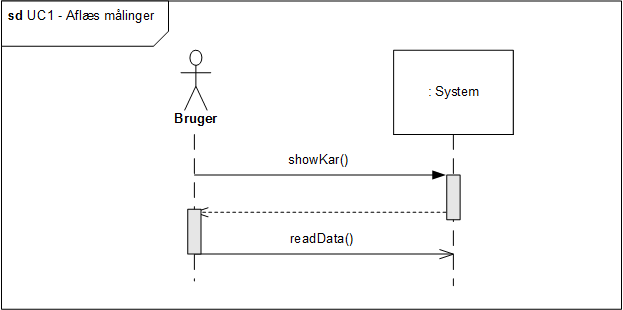
\includegraphics[width=0.8\textwidth]{Systemarkitektur/OverordnedeSekvensdiagrammer/sd_UC1.PNG}
    \caption{sd - Usecase 1}
    \label{fig:sd_UC1}
\end{figure}

\subsection{Overordnet sekvensdiagram for usecase 2 - Manuel vanding}
På diagrammet ses interaktion mellem System og Bruger for usecase 2 - Manuel vanding.

\begin{figure}[H]
    \centering
    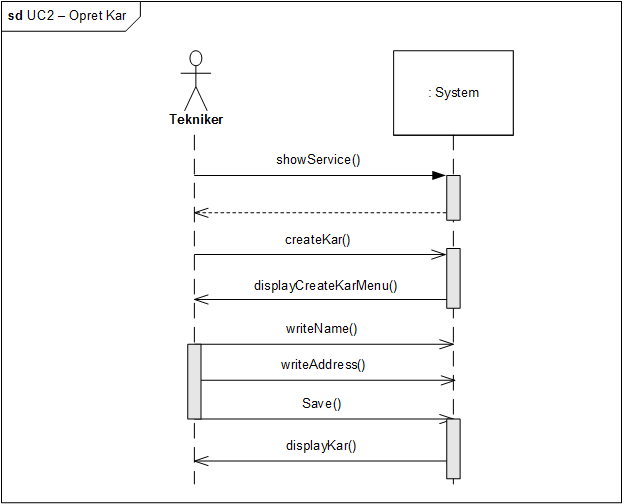
\includegraphics[width=0.8\textwidth]{Systemarkitektur/OverordnedeSekvensdiagrammer/sd_UC2.PNG}
    \caption{sd - Usecase 2}
    \label{fig:sd_UC2}
\end{figure}


\subsection{Overordnet sekvensdiagram for usecase 3 - Indtast pH-værdi}
På diagrammet ses interaktion mellem System og Bruger for usecase 3 - Indtast pH-værdi.

\begin{figure}[H]
    \centering
    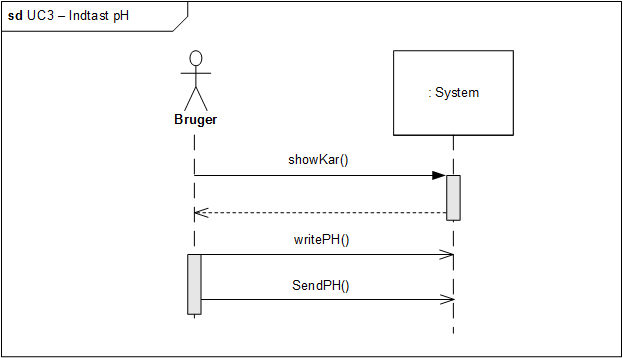
\includegraphics[width=0.8\textwidth]{Systemarkitektur/OverordnedeSekvensdiagrammer/sd_UC3.PNG}
    \caption{sd - Usecase 3}
    \label{fig:sd_UC3}
\end{figure}

\subsection{Overordnet sekvensdiagram for usecase 4 - Indtast volumen}
på diagrammet ses interaktion mellem System og Bruger for usecase 4 - Indtast volumen.

\begin{figure}[H]
    \centering
    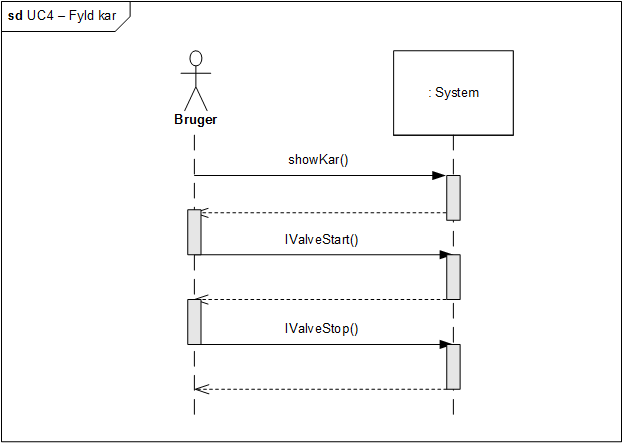
\includegraphics[width=0.8\textwidth]{Systemarkitektur/OverordnedeSekvensdiagrammer/sd_UC4.PNG}
    \caption{sd - Usecase 4}
    \label{fig:sd_UC4}
\end{figure}

\subsection{Overordnet sekvensdiagram for usecase 5 - Opret kar}
På diagrammet ses interaktion mellem System og Tekniker for usecase 5 - Opret kar.

\begin{figure}[H]
    \centering
    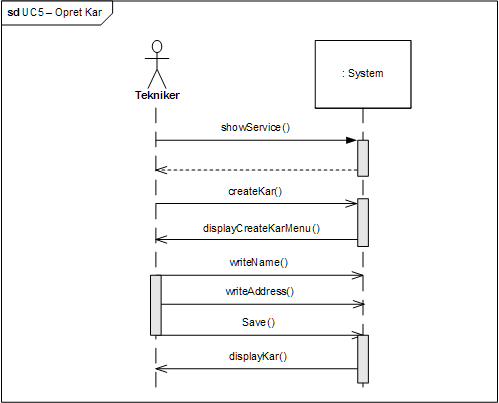
\includegraphics[width=0.8\textwidth]{Systemarkitektur/OverordnedeSekvensdiagrammer/sd_UC5.PNG}
    \caption{sd - Usecase 5}
    \label{fig:sd_UC5}
\end{figure}

\subsection{Overordnet sekvensdiagram for usecase 6 - Slet kar}
På diagrammet ses interaktion mellem System og Tekniker for usecase 6 - Slet kar.

\begin{figure}[H]
    \centering
    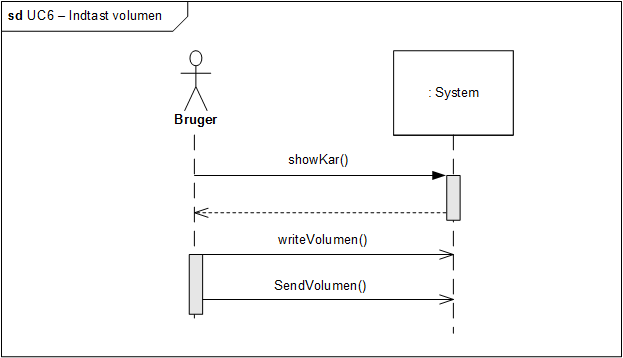
\includegraphics[width=0.8\textwidth]{Systemarkitektur/OverordnedeSekvensdiagrammer/sd_UC6.PNG}
    \caption{sd - Usecase 6}
    \label{fig:sd_UC6}
\end{figure}

\subsection{Overordnet sekvensdiagram for usecase 7 - Kalibrer pH-probe}
På diagrammet ses interaktion mellem System og Tekniker for usecase 7 - Kalibrer pH-probe.

\begin{figure}[H]
    \centering
    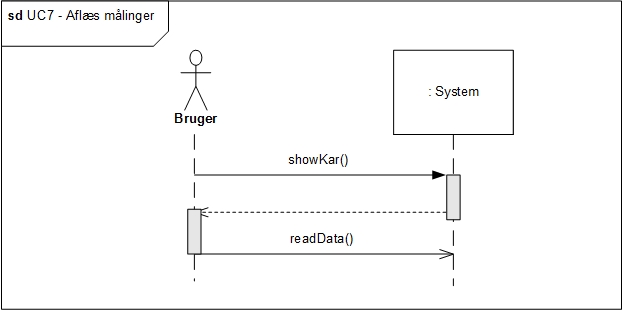
\includegraphics[width=0.8\textwidth]{Systemarkitektur/OverordnedeSekvensdiagrammer/sd_UC7.PNG}
    \caption{sd - Usecase 7}
    \label{fig:sd_UC6}
\end{figure}


\newpage
\section{Klasseidentifikation}
%!TEX root = ../../main.tex

I system domænemodellen, som ses på figur \ref{fig:System_Domain_Model}, kan det ses at der blev identificeret nogle konceptuelle klasser, hvor hver klasse har til ansvar at løse et specifikt problem. Ud fra dette vil vi gerne se på hvilke domæner og grænseflader der er. Hvor grænsefladerne er det der skal anvendes når dele af systemmet skal kommunikerer og domæne står for de resterende problemer. Så ud fra domænemodellen er følgende grænseflade- og domæneproblemer defineret:
\begin{itemize}
	\item Grænseflader:
		\begin{itemize}
			\item Bruger Grænseflade
			\item GUI grænseflader
			\item FlexPMS grænseflader 
			\item Kar grænseflader
			\item SensorØ grænseflader
		\end{itemize}
	\item Domæne:
	\begin{itemize}
			\item Håndtering af de forskellige setværdier (pH, volumen, jordfugtighed osv.)
			\item Håndtering af målinger
			\item Håndtering af Kar data 
			\item Håndtering af SensorØ data 
		\end{itemize}
\end{itemize} 

Ud fra dette udarbejdes applikationsmodeller. Hver applikationsmodel har til opgave at vise de klasser som er involveret i de forskellige use cases. Dette håndteres af kontrolklassen. grænseflade- og domæneklasserne er bestem ud fra det overstående så der er identificeret følgende klasser:

\begin{itemize}
	\item Boundaryklasser:
		\begin{itemize}
			\item \textbf{GUI} - Brugergrænseflade mellem bruger og system
			\item \textbf{Database} - Grænseflade mellem GUI og FlexPMS
			\item \textbf{Protokol} - Bussystemerne der kommunikere med vores hardware 
		\end{itemize}
	\item Domainklasser:
	\begin{itemize}
			\item \textbf{Sensor} - Måler de forskellige data (pH, volumen, jordfugtighed osv.)
			\item \textbf{Kar} - Håndterer de specifikke data for de individuelle kar
			\item \textbf{SensorØ} - Håndterer de specifikke data for de individuelle SensorØ'er
	\end{itemize} 
\end{itemize} 
 
Ud fra use casene og de definerede klasser, kan der nu oprettes applikationsmodeller. Applikationsmodellerne
består af henholdsvis en kontrolklasse der varetager use casens forløb, samt de definerede domain-
og boundaryklasser, som kontrolklassen skal bruge for at opfylde dette. Da der er mange af use casene der ligner hinanden er nogle af dem slået sammen i en applikationsmodel. 


\subsection{Klassediagram for use case 7 - Aflæs data}

\begin{figure}[H]
    \centering
    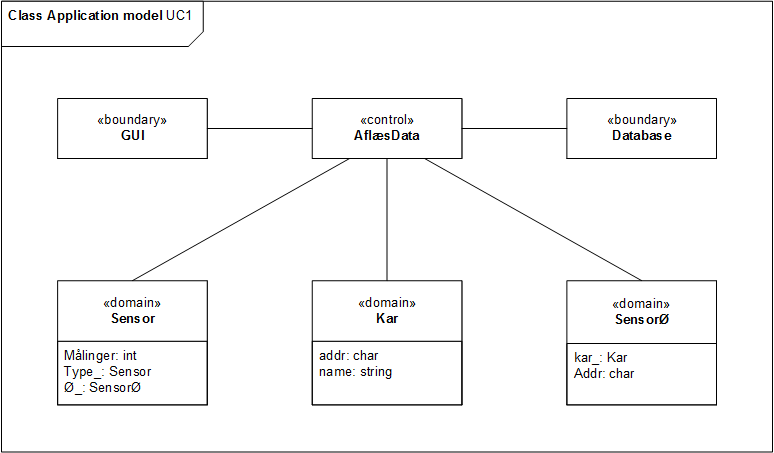
\includegraphics[width=0.8\textwidth]{Systemarkitektur/KlasseDiagrammer/7_AflaesData.png}
    \caption{Applikationsmodel for UC1}
    \label{fig:app_uc7}
\end{figure}

Dette klassediagram er benyttet til at identificere nødvendige klasser for at udføre use case 7.
Nedenfor er beskrives kort klassernes ansvar for use case 7.
\\\\
\textbf{AflæsData:}\\
varetager og koordinerer interaktionen mellem de interne klasser i henhold til use casen.
\\\\
\textbf{GUI:}\\
Grænseflade mellem, system go bruger, hvor brugeren aflæser de målte data. 
\\\\

\subsection{Klassediagram for use case 8 - Manuel vanding}
\begin{figure}[H]
    \centering
    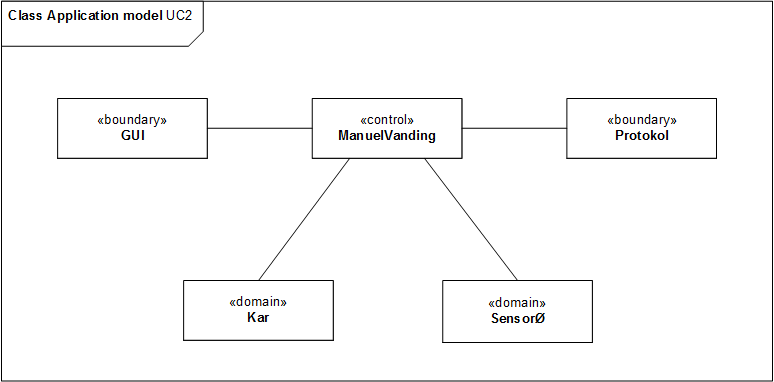
\includegraphics[width=0.8\textwidth]{Systemarkitektur/KlasseDiagrammer/8_ManuelVanding.png}
    \caption{Applikationsmodel for UC8}
    \label{fig:app_uc8}
\end{figure}

Dette klassediagram er benyttet til at identificere nødvendige klasser for at udføre use case 8.
Nedenfor er beskrives kort klassernes ansvar for use case 8.
\\\\
\textbf{Manuel vanding:}\\
varetager og koordinerer interaktionen mellem de interne klasser i henhold til use casen.
\\\\
\textbf{GUI:}\\
Grænseflade mellem, system go bruger, hvor brugeren kan aktivere den manuelle vanding. 
\\\\
\textbf{Protokol:}\\
Bussystem, der kommunikerer med vores hardware, så manuel vanding kan aktiveres.
\\\\

\subsection{Klassediagram for use case 5 og 6 - Indtast data}

\begin{figure}[H]
    \centering
    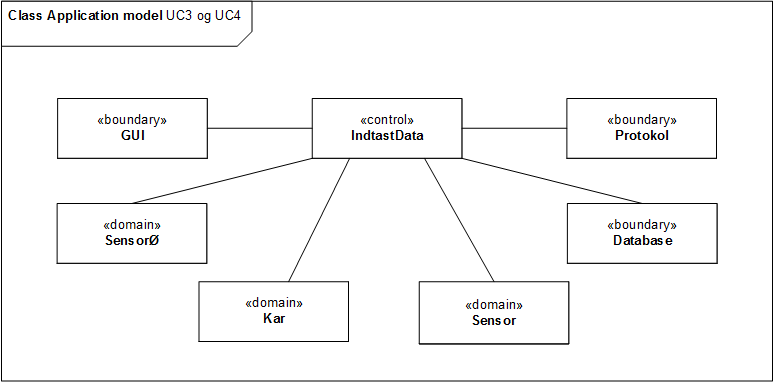
\includegraphics[width=0.8\textwidth]{Systemarkitektur/KlasseDiagrammer/5+6_IndtastData.png}
    \caption{Applikationsmodel for UC5 og UC6}
    \label{fig:app_uc56}
\end{figure}

Dette klassediagram er benyttet til at identificere nødvendige klasser for at udføre use case 5 og 6.
Nedenfor er beskrives kort klassernes ansvar for use case 5 og 6.
\\\\
\textbf{IndtastData:}\\
varetager og koordinerer interaktionen mellem de interne klasser i henhold til use casen.

\textbf{GUI:}\\
Grænseflade mellem, system go bruger, hvor brugeren Indtaste de ønskede data. 
\\\\

\textbf{Database:}\\
Grænseflade mellem GUI og FlexPMS, hvor de  indtastede data bliver gemt. 
\\\\

\subsection{Klassediagram for use case 2 og 10 - Kar manipulation}

\begin{figure}[H]
    \centering
    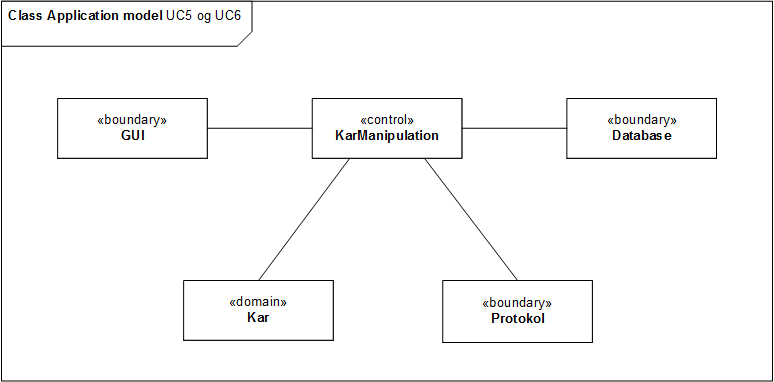
\includegraphics[width=0.8\textwidth]{Systemarkitektur/KlasseDiagrammer/2+10_KarManipulate.png}
    \caption{Applikationsmodel for UC2 og UC10}
    \label{fig:app_uc210}
\end{figure}

Dette klassediagram er benyttet til at identificere nødvendige klasser for at udføre use case 2 og 10.
Nedenfor er beskrives kort klassernes ansvar for use case 2 og 10.
\\\\
\textbf{KarManipulation:}\\
Varetager og koordinerer interaktionen mellem de interne klasser i henhold til use casen.
\\\\
\textbf{GUI:}\\
Grænseflade mellem, system go bruger, hvor brugeren kan oprette og slette kar. 
\\\\

\textbf{Database:}\\
Grænseflade mellem GUI og FlexPMS, hvor det forskellige kar bliver gemt med deres data. 
\\\\

\newpage
\section{Grænsefladebeksrivelser}
%!TEX root = ../../main.tex

\subsection{Ventilstyring Grænsefladebeskrivelse}

Ventilstyring er en grænseflade til systemet, modulet omsætter digital styring fra PSoC'en til analog aktuation i mangetventilen der kontrollerer vandtilførsel, udledning, samt dosering ved karret. 
Modulet tager, som input, et digitalt signal 0-5V. Dette omsættes til analog styring af ventilen. 
Derudover tilføres kontrolkredsen 12V som forsyningsspænding. fig.\ref{screenshot:tabel1},s.\pageref{screenshot:tabel1}

\begin{figure}[H]
	\centering
	\includegraphics[scale=0.6]{../Projektdokumentation/Systemarkitektur/Graenseflader/Screenshots/tabel1}
	\caption{Grænsefladebeskrivelse: Ventilstyring}
	\label{screenshot:tabel1}
\end{figure}


\subsection{Doseringspumpe Grænsefladebeskrivelse}

Doseringspumpen er ligeledes en grænseflade til systemet, modulet omsætter et digital PWM-signal fra PSoC'en til en procentvis styring af doseringspumpen så den kan kører i flere etaper. Modulet tager, som input, et digitalt PWM-signal 0-5V. Dette omsættes til analog styring i doseringspumpen. 
Derudover tilføres kontrolkredsen 12V som forsyningsspænding. fig.\ref{screenshot:tabel2},s.\pageref{screenshot:tabel2}  

\begin{figure}[H]
	\centering
	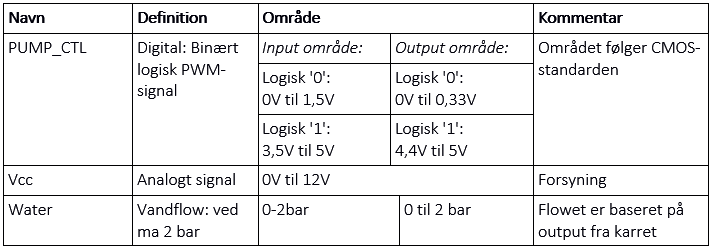
\includegraphics[scale=0.6]{../Projektdokumentation/Systemarkitektur/Graenseflader/Screenshots/tabel2_Pumpe}
	\caption{Grænsefladebeskrivelse: Doseringspumpe}
	\label{screenshot:tabel2}
\end{figure}


\subsection{Flowsensor Grænsefladebeskrivelse}
Flowsensor fungerer som grænseflade til systemet, modulet omsætter vandflow i sensoren til et digital PWM-signal der angiver hvor meget vand der flyder igennem sensoren. Modulet forsynes med +5V forsyning, samt GND, og afgiver PWM-signal 
Dette PWM omsættes via et eksternt counterkredsløb til at give logisk '1' ved hver 10. count. Dette trækker et interrupt i PSoC'programmet.fig.\ref{screenshot:tabel3},s.\pageref{screenshot:tabel3}

\begin{figure}[H]
	\centering
	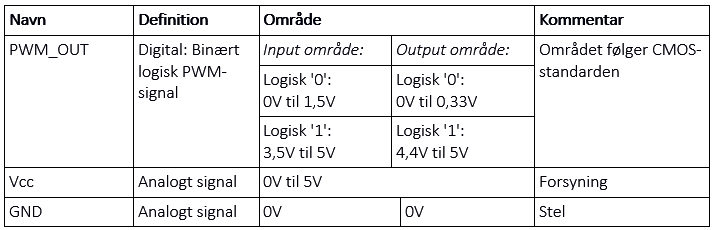
\includegraphics[scale=0.6]{../Projektdokumentation/Systemarkitektur/Graenseflader/Screenshots/tabel3_Flowsensor}
	\caption{Grænsefladebeskrivelse: Flowsensor}
	\label{screenshot:tabel3}
\end{figure}

\subsection{PSU (Power Supply Unit) Grænsefladebeskrivelse}
Strømforsyningen har til formål at forsyne hele systemet med både 5V og 12V. Den genererer disse spændinger ud fra el-nettets 230VAC.

\begin{table}[h]
\centering
\begin{tabular}{|l|l|l|l|}
\hline
\textbf{Navn} & \textbf{Definition} & \textbf{Område} & \textbf{Kommentar} \\ \hline
5V            & Analogt signal      & 0-5V            & Forsyning          \\ \hline
12V           & Analogt signal      & 0-12V           & Forsyning          \\ \hline
GND           & Analogt signal      & 0V              & Stel               \\ \hline
\end{tabular}
\end{table}